
\item A block of mass \(0.18 \, \text{kg}\) is attached to a spring of force-constant \(2 \, \text{N/m}\). The coefficient of friction between the block and the floor is \(0.1\). Initially the block is at rest and the spring is un-stretched. An impulse is given to the block as shown in the figure. The block slides a distance of \(0.06 \, \text{m}\) and comes to rest for the first time. The initial velocity of the block in m/s is \(V = N/10\). Then \(N\) is \underline{\hspace{2.5cm}}.
    \begin{center}
        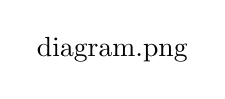
\begin{tikzpicture}
            \node at (0, 0) {diagram.png};
        \end{tikzpicture}
    \end{center}
